\section{Simulator Evaluation}

\subsection{Overall System}
\begin{enumerate}
	\item It works on other machines first run, (different machine different gpu). Verify it works on WSL?
	\item Get benchmark of the system i.e GPU usage and CPU usage.
\end{enumerate}

\subsection{Tracking System}
\subsubsection{Together}
\begin{enumerate}
	\item Mention lighting issues.
\end{enumerate}

\begin{figureBox}[label={fig:framerate-overall}, width=1.0\linewidth]{Overall Framerate}
	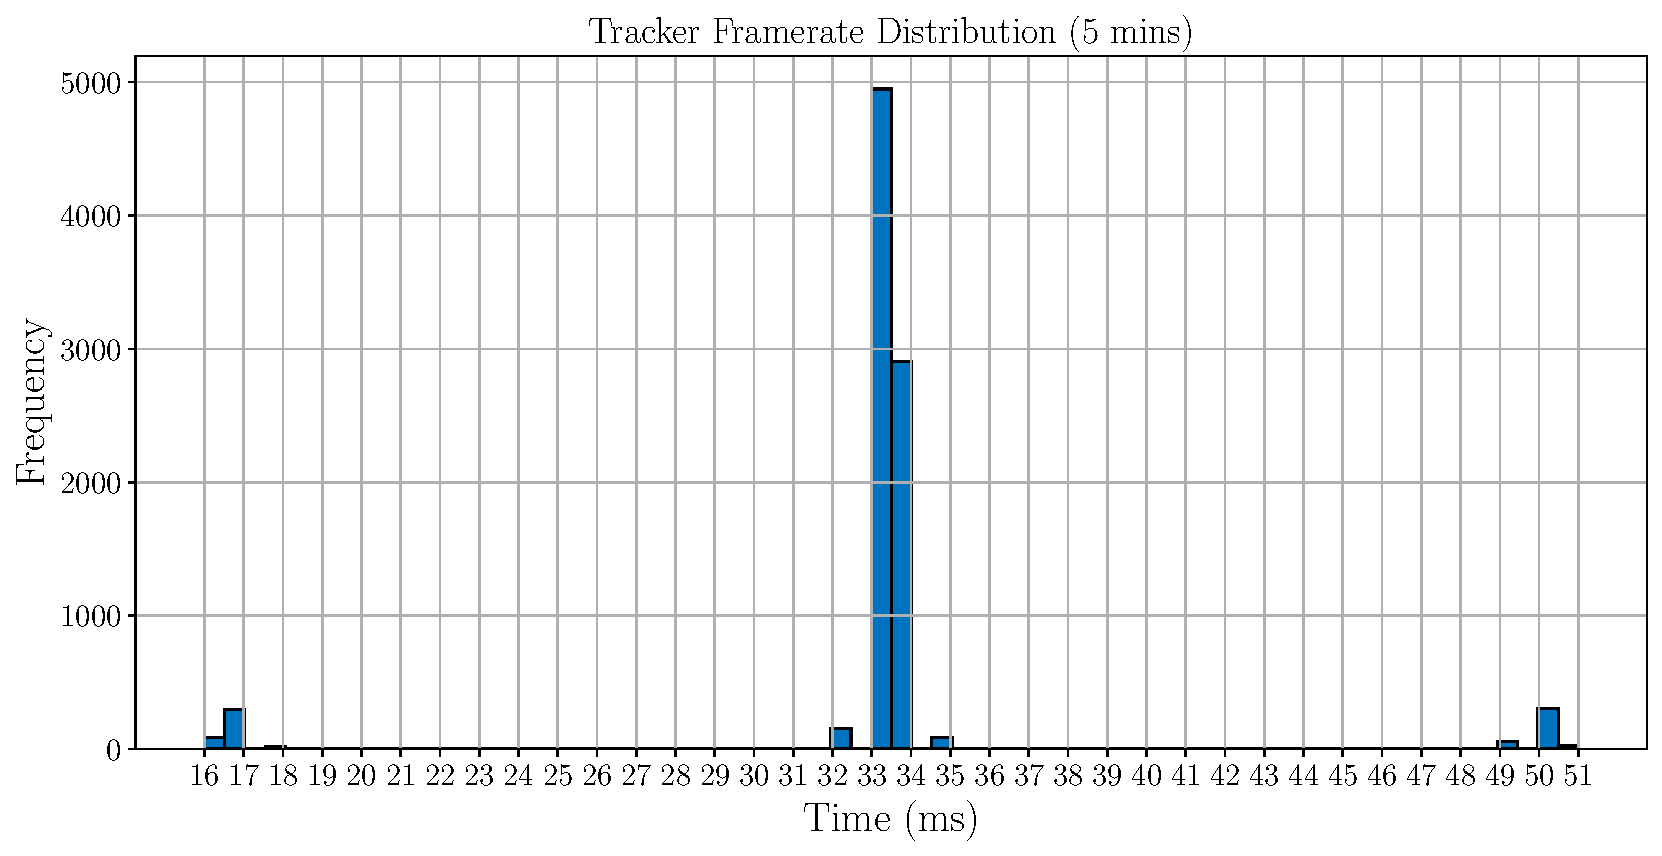
\includegraphics[width = 1.0\linewidth]{./evaluation/figures/framerate-overall.pdf}
\end{figureBox}

As can be seen in Figure \ref{fig:framerate-overall}, the framerate of the system is quite low. 90.83\% of the time the framerate is between 30 and 35ms. There is what at first glance a strange phenomenon of a group of latencies at 16-18ms (4.46\%) and 49-51ms (4.39\%). This is due to the framerate of the renderer, as it lazily converted on request it basically chunked to the nearest 1000/60 = 16.666. Even though the tracker is running at 30fps, it is possible to have a latency of 16ms if the tracker fails to the meet the 30fps requirement for a frame buffering the result for the next frame. This means the next capture is already ready by the next frame so it makes it appear like the camera has a higher framerate than 30. \textcolor{red}{rewrite this in a less shit way}

We investigated down scaling the image to increase performance. We only found that down scaling it once was enough to get the performance we needed. Down scaling it further did not offer any significant performance increases and significantly decreased tracking quality. As can be seen in Figure \ref{fig:pydown}, the performance of the system increases noticeably between going from 2048 x 1536 to 1024 x 793 but reducing the resolution further does not provide any speed benefit at all as we are already running at 30fps which is the cameras refresh rate.

\begin{figureBox}[label={fig:pydown}, width=1.0\linewidth]{Comparing Resolutions}
	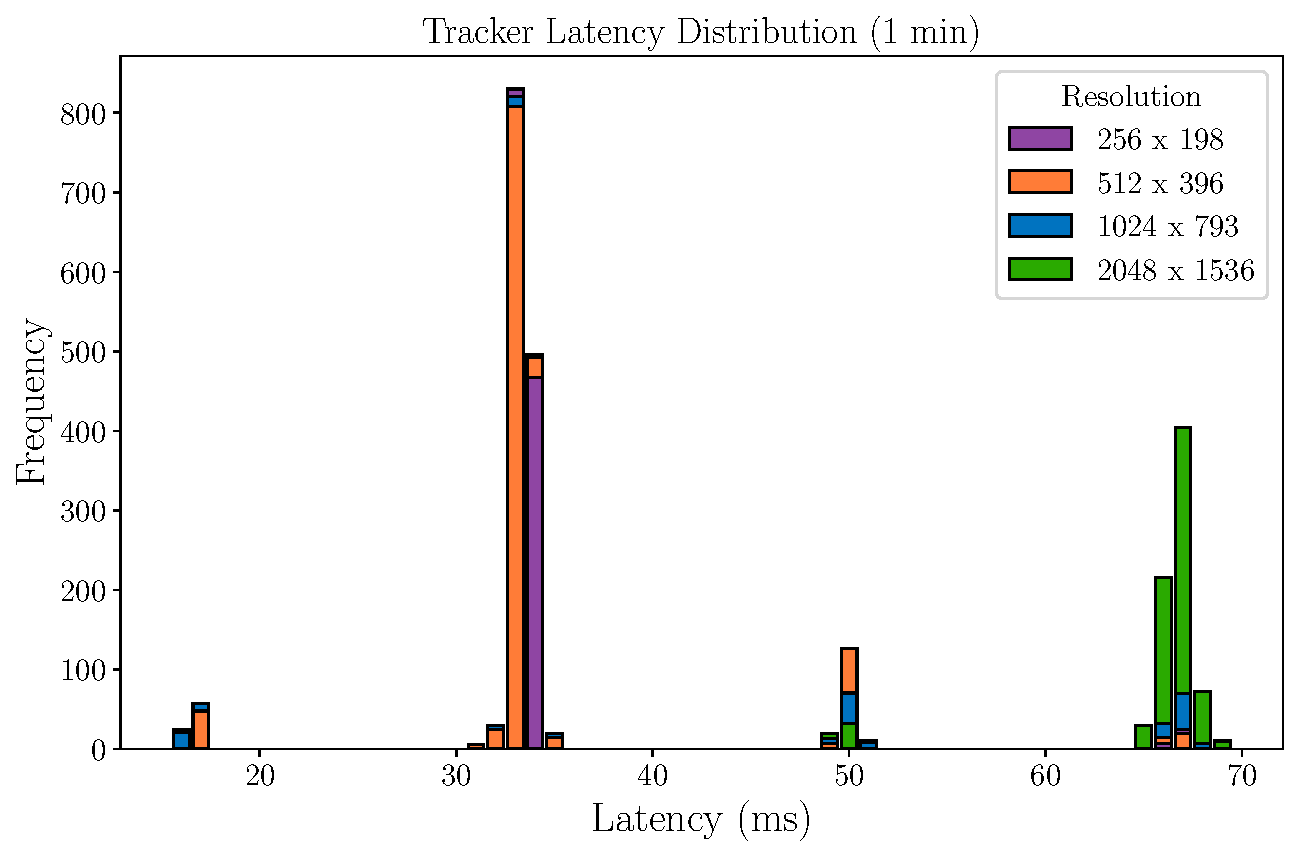
\includegraphics[width = 1.0\linewidth]{./evaluation/figures/pydown.pdf}
\end{figureBox}

As can be seen in Figure \ref{fig:process-times-distributions}, of the three separate threads (captures from the kinect camera, tracking the hand and eye, and rendering with OpenGL) which are running at the same time, the bottleneck is waiting for the kinect camera to return the capture. This means there isn't any benefit to speeding up the tracking algorithm.

\begin{figureBox}[label={fig:process-times-distributions}, width=1.0\linewidth]{Comparing Processing Times}
	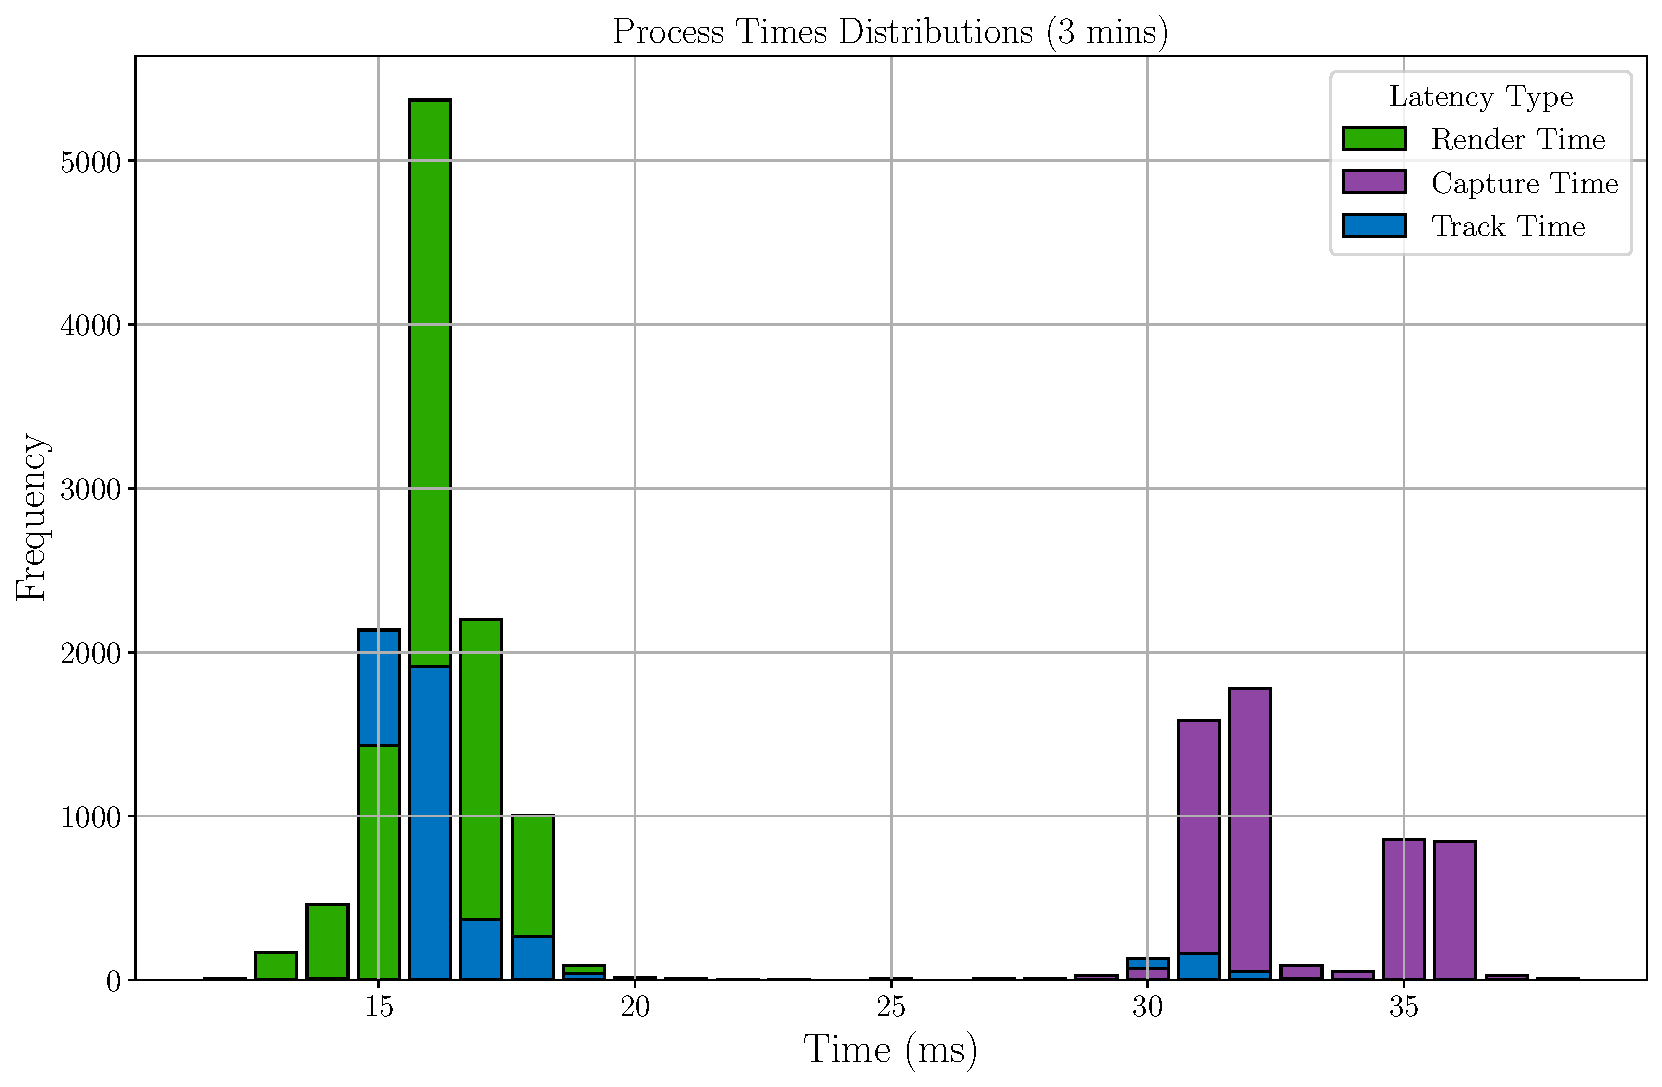
\includegraphics[width = 1.0\linewidth]{./evaluation/figures/process-times-distributions.pdf}
\end{figureBox}.

\textcolor{red}{Estimate Latency, 12.8 exposure which you should cite, plus workout how the framerate effects it + 15 ms for tracking plus work out how the random chance of being selected during rendering works and compare to it similar systems like oculus quest and maybe fishbowl and vision pro?} 

\subsubsection{Head Tracking}
\begin{enumerate}
	\item Measure accuracy by moving head around and seeing how often it loses track at different distances. While facing camera. Test with glasses on?
	\item Measure the angle of the head where the tracker stops working.  
\end{enumerate}

%TODO

\begin{figureBox}[label={fig:angle-setup}, width=1.0\linewidth]{Angle Setup}
	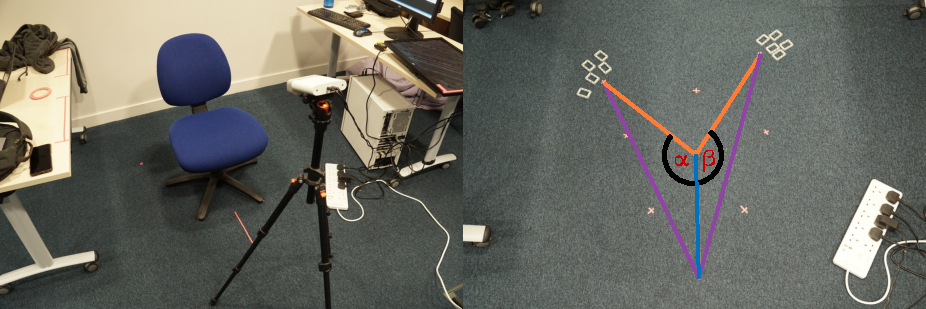
\includegraphics[width = 1.0\linewidth]{./evaluation/figures/angle-setup.pdf}
\end{figureBox}

%TODO

\begin{figureBox}[label={fig:head-angle}, width=0.7\linewidth]{Angle of failure for headtracking}
	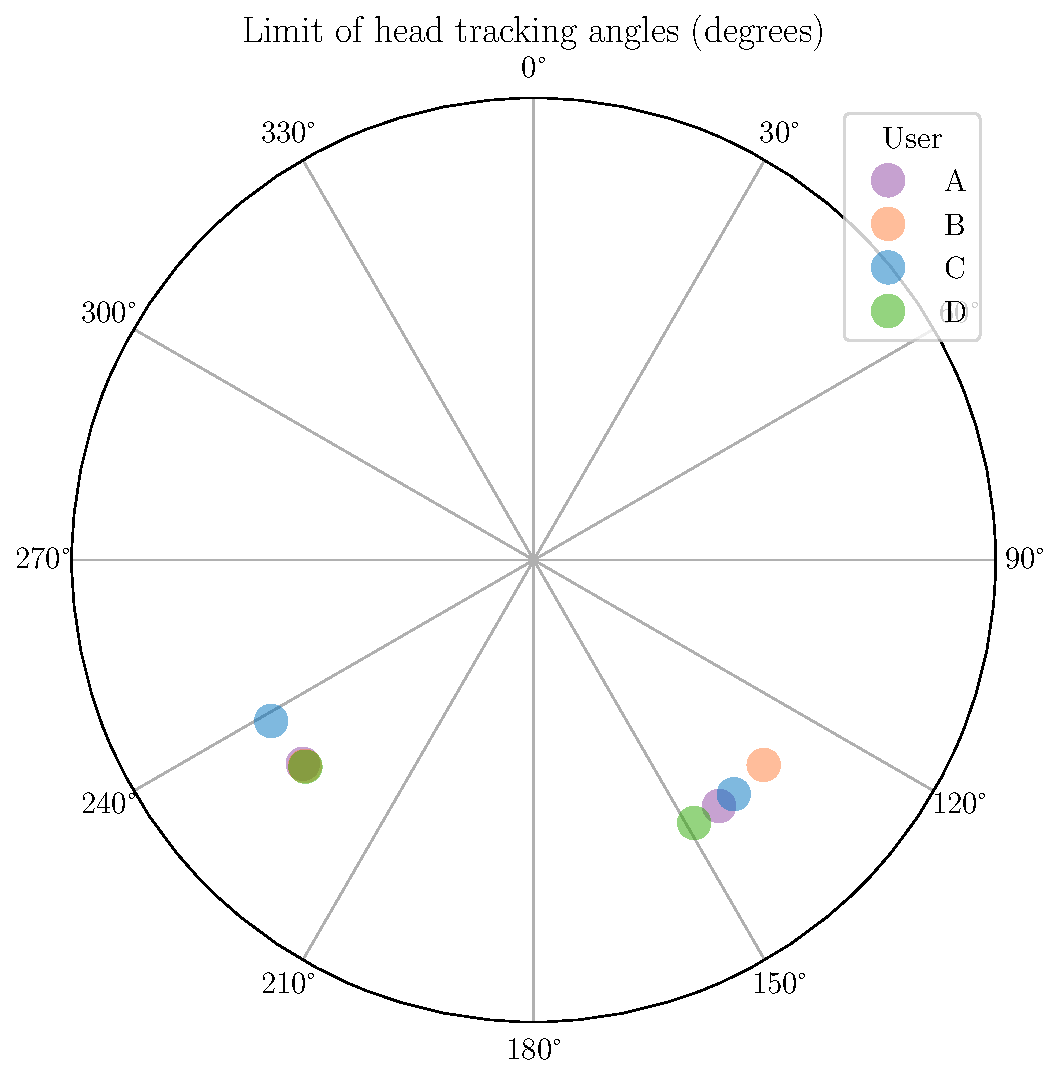
\includegraphics[width = 1.0\linewidth]{./evaluation/figures/user-angles.pdf}
\end{figureBox}

%TODO

\begin{figureBox}[label={fig:incorrect-head-track}, width=0.7\linewidth]{Incorrect Head Tracking}
	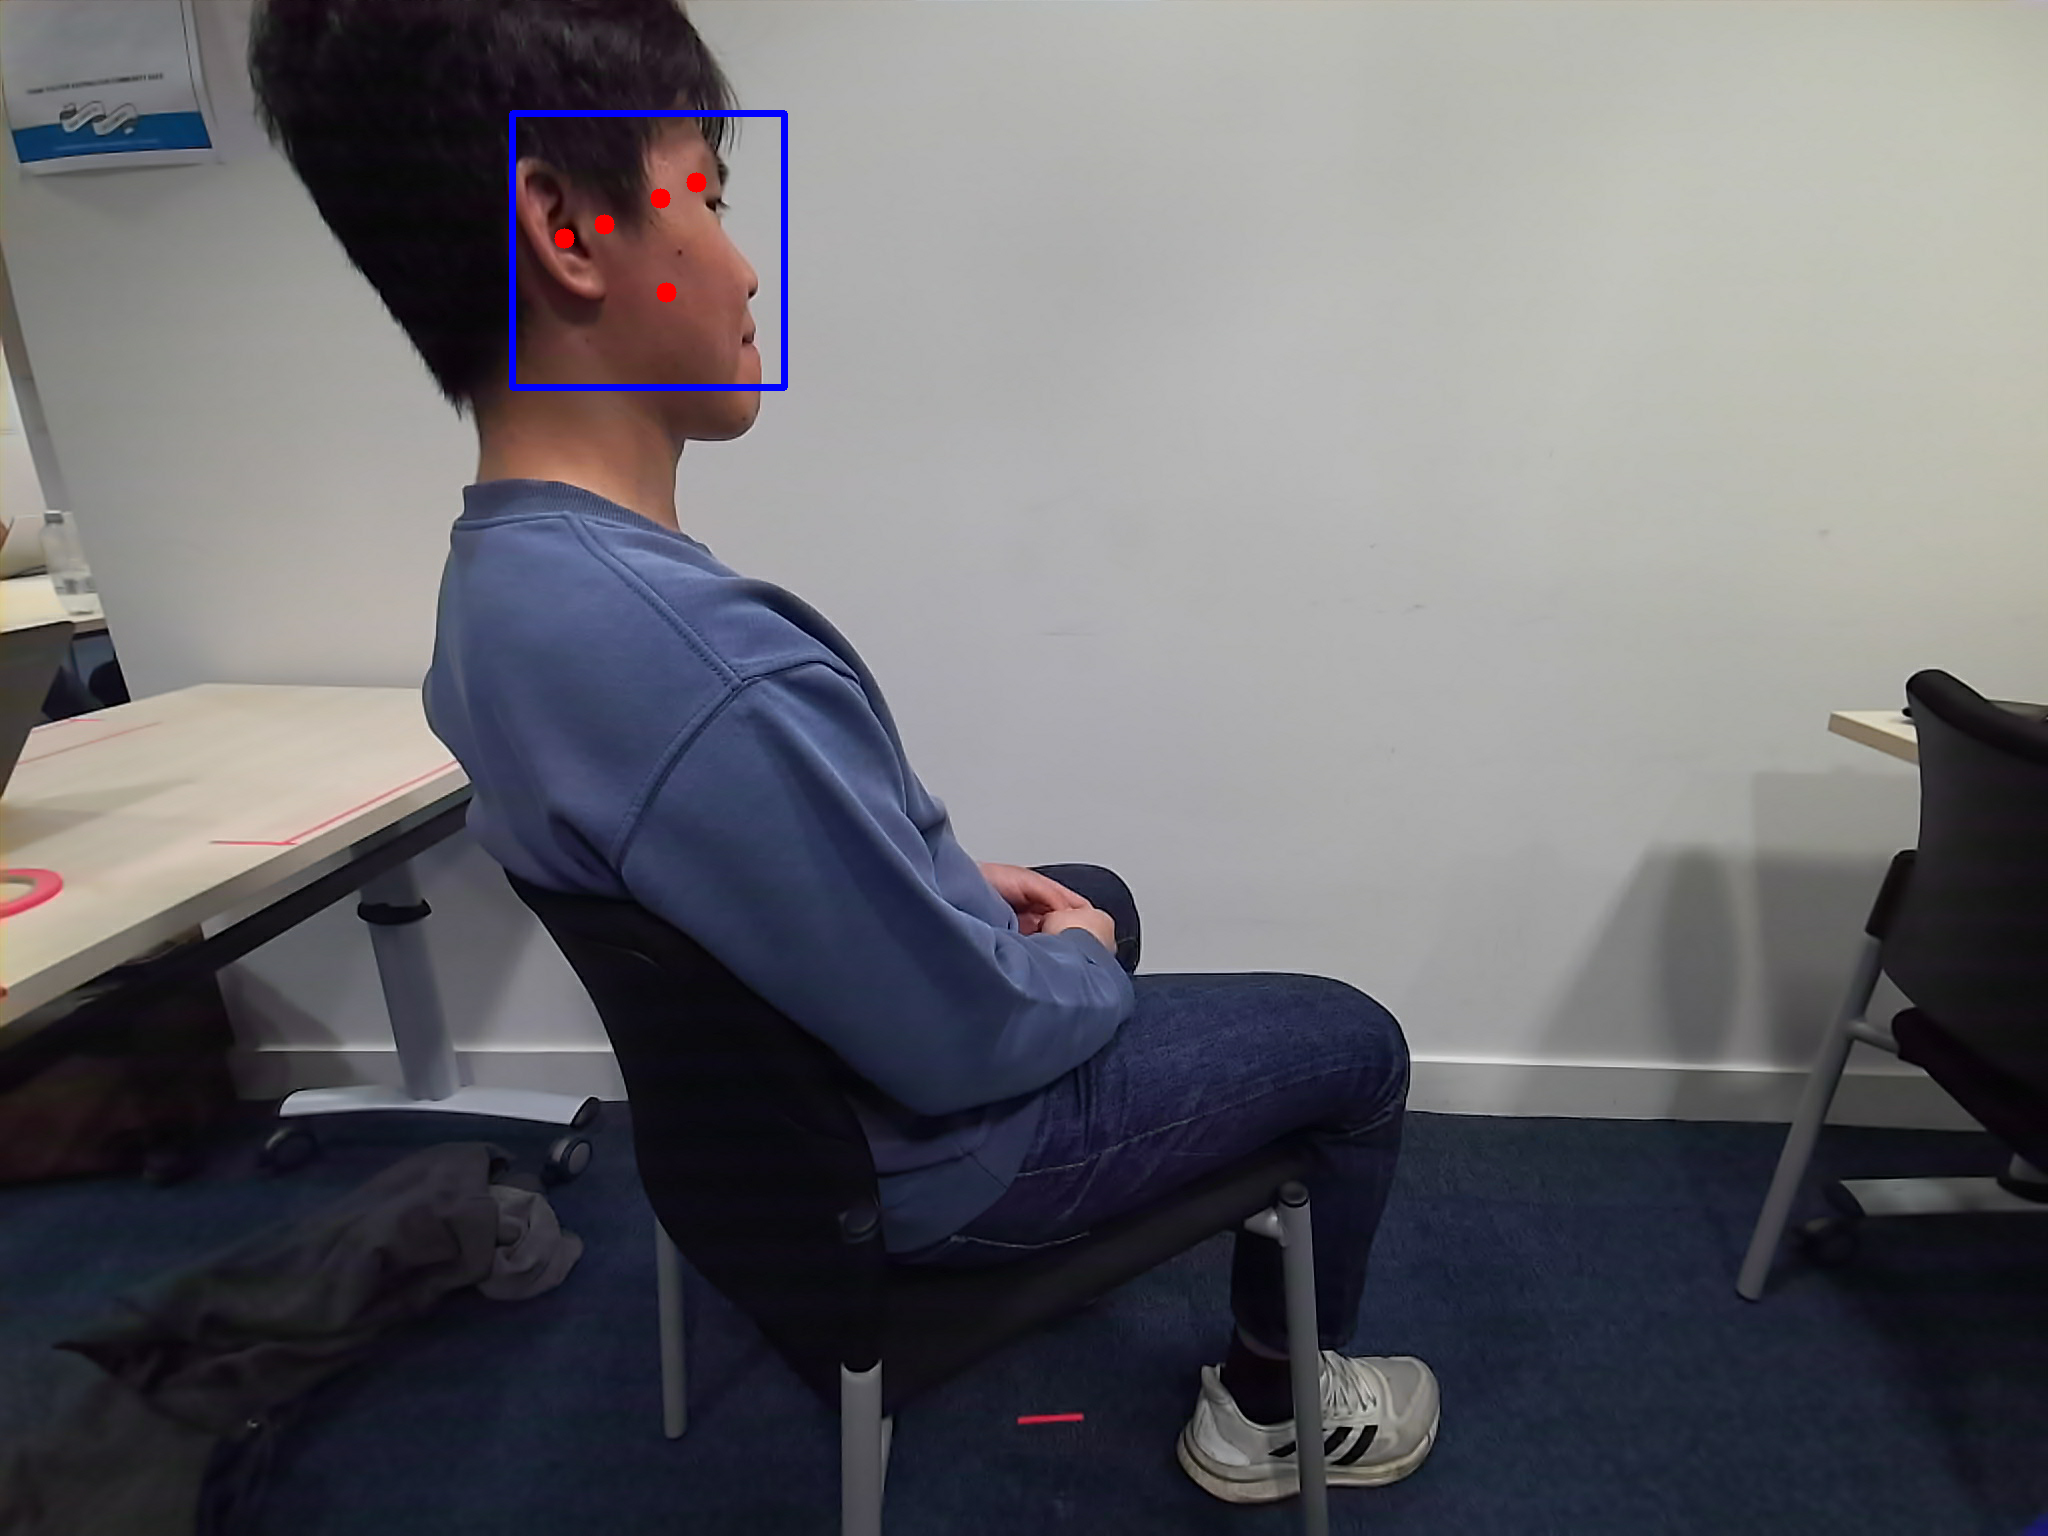
\includegraphics[width = 1.0\linewidth]{./evaluation/figures/incorrectTrackedFace.png}
\end{figureBox}

%TODO

\begin{figureBox}[label={fig:distance-setup}, width=0.7\linewidth]{Setup for distance testing}
	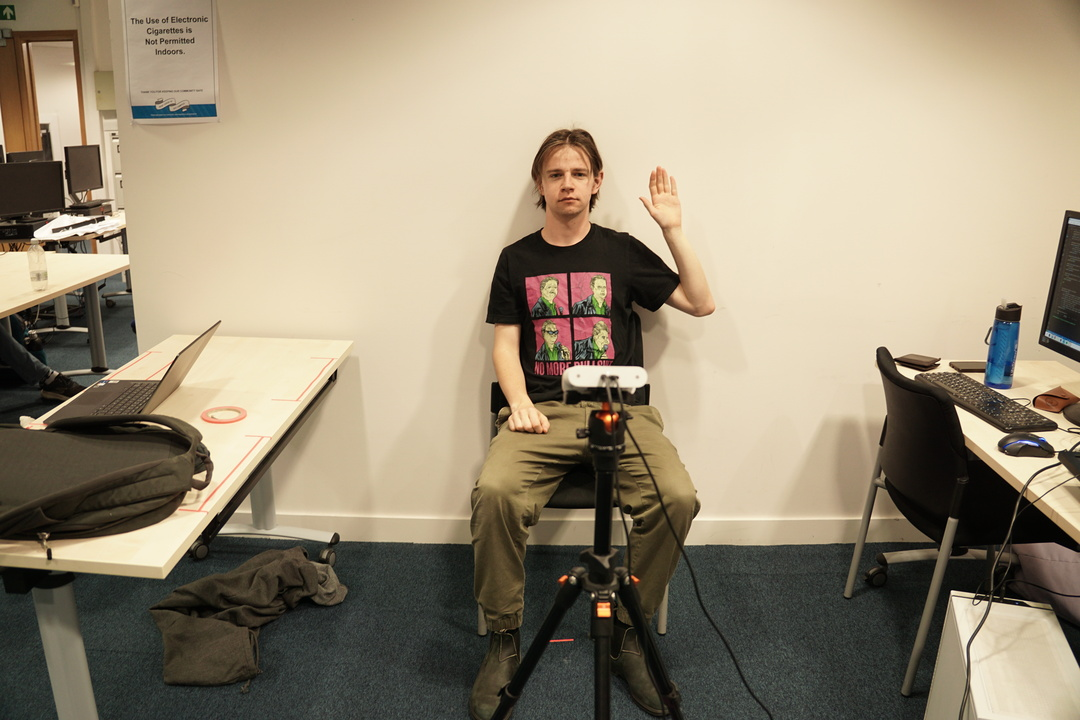
\includegraphics[width = 1.0\linewidth]{./evaluation/figures/distance_setup.jpg}
\end{figureBox}

%TODO

\begin{figureBox}[label={fig:track-distance}, width=1.0\linewidth]{Tracking success rate at different distances}
	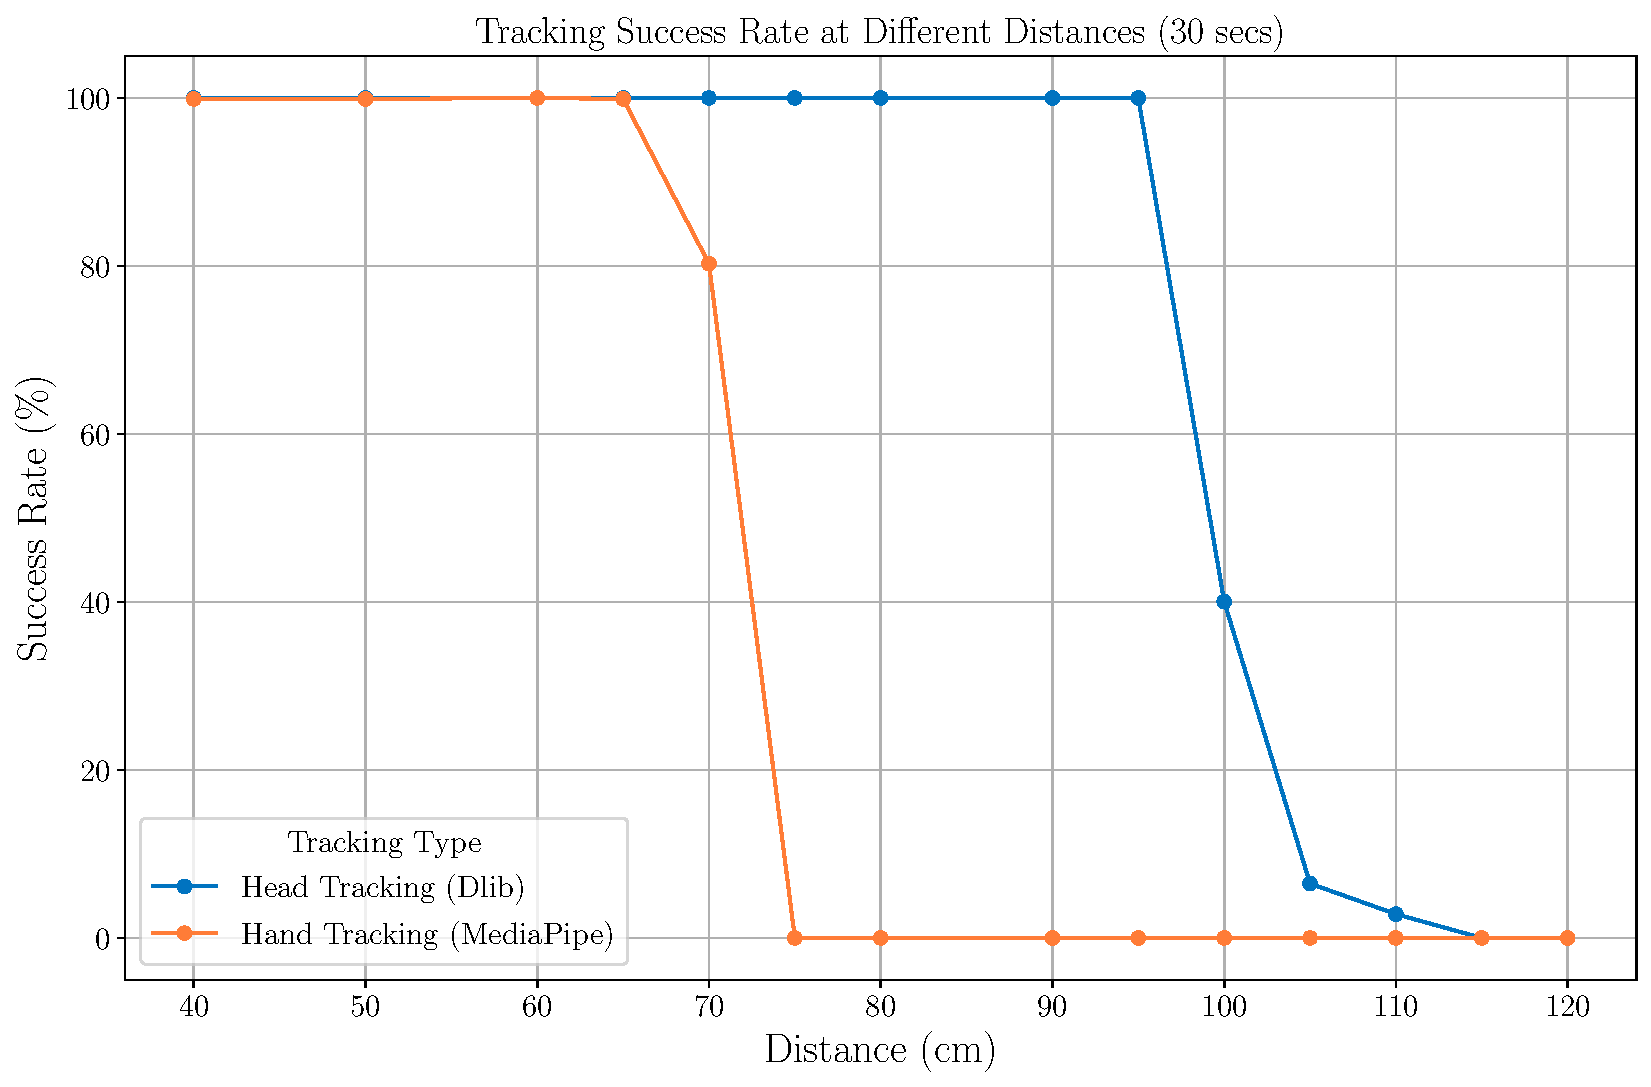
\includegraphics[width = 1.0\linewidth]{./evaluation/figures/tracking-success-rate.pdf}
\end{figureBox}

\textcolor{red}{mention thing ed talked about how it's probably just due to the training data of the model resulting in the real quick drop off, don't forget this is measured from the front of the chair so add and extra 50cm is there and it's to the tripod base not the camera so probably an extra 15cm}
%TODO

\subsubsection{Hand tracking}
\begin{enumerate}
	\item Estimate throughput via logging (unique points). Draw a bell curve like graph of the time between each result from the tracker.
	\item Measure accuracy by moving head around and seeing how often it loses track at different distances. Change hand orientations
	\item Mention occlusion issue. 
	\item Wall vs no wall issue. 
	\item The colour of the screen also affects the hand tracker. 
	\item Maybe should have added image segmentation model to make the hand tracker better.
\end{enumerate}

\subsection{Renderer}
\textcolor{red}{TODO}
\begin{enumerate}
	\item Talk about and give an image of the rendering system displaying a complex scene.
	\item Get framerate?
\end{enumerate}

We wanted to evaluate how accurate our rendering system. As our rendering system propose is to create the illusion of 3D objects in the real world, we wanted to see how well it could recreate a real object. We chose a cube as it is a simple object that is easy to recreate. We created a physical cube out of lego and created a virtual cube in our simulator both with the same dimensions of 13.5cm x 13.5cm x 12cm as can be seen in Fig~\ref{fig:real-vs-rendered}.

\begin{figureBox}[label={fig:real-vs-rendered}, width=1.0\linewidth]{A real and rendered cube}
	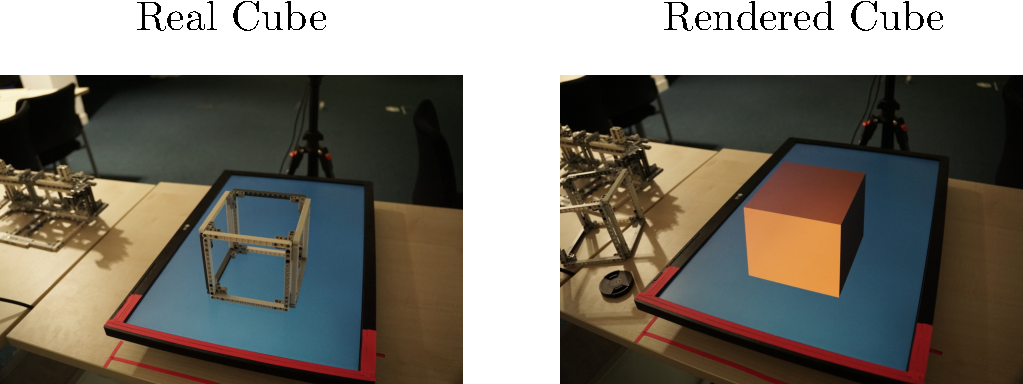
\includegraphics[width = 1.0\linewidth]{./evaluation/figures/real-vs-rendered.pdf}
\end{figureBox}

Because the physical cube is hollow this allowed us to easily to compare the two cubes by superimposing them. We tested a variety of different perspectives and verified that the two cubes were indeed the same size and shape and completely overlapped. Some examples can be seen in Fig~\ref{fig:super-imposed}, it is worth noticing that the images might be slightly off as the system was tracking my eye and not the camera lense which was both below and about 10cm in front of my eye. This shows that our rendering system is accurate and can be used to create the illusion of 3D objects in the real world. 

\begin{figureBox}[label={fig:super-imposed}, width=1.0\linewidth]{Superimposed real and rendered cube}
	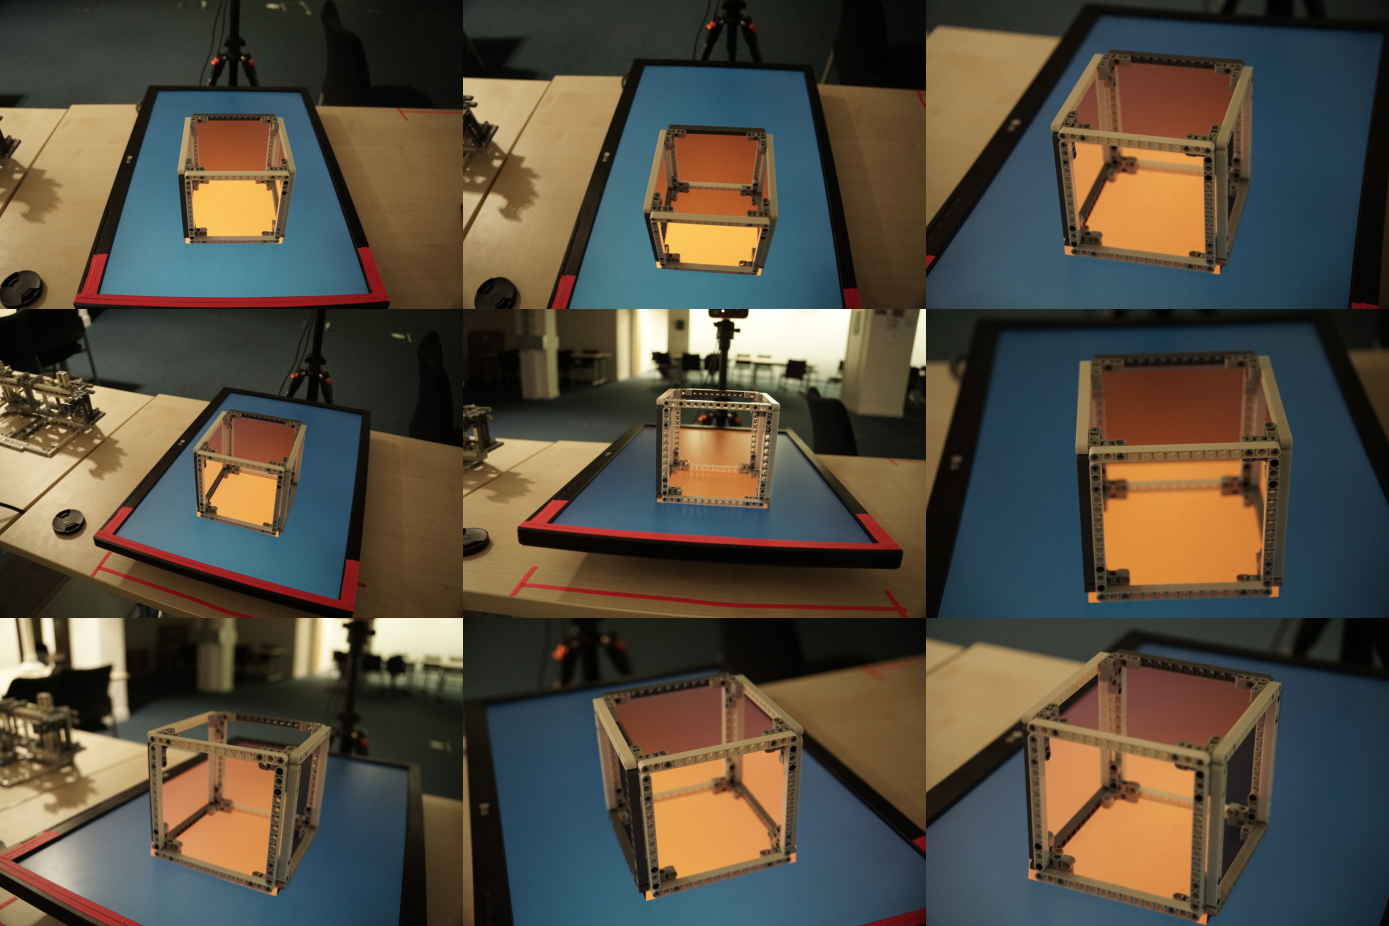
\includegraphics[width = 1.0\linewidth]{./evaluation/figures/super-imposed.pdf}
\end{figureBox}
